% no answer key
% \documentclass[letterpaper]{exam}

% answer key
\documentclass[letterpaper, landscape]{exam}
\usepackage{2in1, lscape} 
\printanswers{}

\usepackage{units} 
\usepackage{xfrac} 
\usepackage[fleqn]{amsmath}
\usepackage{cancel}
\usepackage{float}
\usepackage{mdwlist}
\usepackage{booktabs}
\usepackage{cancel}
\usepackage{polynom}
\usepackage{caption}
\usepackage{fullpage}
\usepackage{comment}
\usepackage{enumerate}
\usepackage{graphicx}
\usepackage{parskip}

\everymath{\displaystyle}

% the textcent command eats the space following the symbol
\usepackage{xspace}
\newcommand{\cent}{\textcent\xspace}

\title{Statistics \\ Homework Eleven}
\date{\today}
\author{}

\begin{document}

  \maketitle

  \section{Homework}
  \ifprintanswers{}
  \else
    \begin{itemize*}
      \item read Chapter 12 
      \item exercises: 27--32, 34--40, 44--51, 54--56
    \end{itemize*}
  \fi

  \ifprintanswers{}
    \begin{description}

      \item[27] 
        The probability of each bet losing is 0.75. Since the bets are
        independent, the probability of all 8 losing is
        \[
          p_{fail} = 0.75^8 \approx \boxed{ 0.1001 }
        \]

      \item[28]
        There is a 92.8\% chance of a person not being a universal donor. The
        probability one of the 10 being a universal donor is:
        \[
          p = 1 - 0.928^{10} \approx \boxed{ 0.5263 }
        \]

      \item[29]
        \begin{enumerate}[(a)]
          \item 
            \[
              \frac{9}{20} \cdot \frac{1}{20} \cdot \frac{1}{20} 
                \approx \boxed{ 0.0011 }
            \]

          \item
              The probability that wheel 1 and exactly one of the other two
              wheels both show a cherry is:
              \[
                \frac{9}{20} \cdot \frac{1}{20} \cdot \frac{19}{20} 
                  \approx \boxed{ 0.0214 }
              \]

              The probability that wheel 1 doesn't show a cherry and wheels 2 and 3 
              do is:
              \[
                \frac{11}{20} \cdot \frac{1}{20} \cdot \frac{1}{20} 
                  \approx \boxed{ 0.0014 }
              \]

            \item
              Since the probabilities are mutually exclusive, you can add them:
              \[
                p \approx 2 \cdot 0.0214 + 0.0014 \approx \boxed{ 0.0441 } 
              \]
        \end{enumerate}

      \item[30]
        \begin{enumerate}[(a)]
          \item 
            \[
              p_{up} = 0.65^3 \approx \boxed{ 0.2746 }
            \]

          \item 
            The probability it goes down for 3 years in a row is:
            \[
              p_{down} = 0.35^3 \approx 0.0429
            \]

            The probability of 3 consecutive years of either loss or gain is:
            \[
              p \approx 0.2746 + 0.0429 = \boxed{ 0.3175 }
            \]

        \end{enumerate}

      \item[31]
        \begin{enumerate}[(a)]
          \item The probability that neither one admits him is:
            \[
              p_{reject} = 0.6 \cdot 0.5 = \boxed{ 0.3 }
            \]

            Another way to figure this out is to find the probability that he
            gets in to either one and then subtract this from 1:
            \begin{align*}
              p_{accept} & = 0.4 + 0.5 - 0.4 \cdot 0.5 = 0.7 \\
              p_{reject} & = 1 - p_{accept} \\
                         & = 1 - 0.7 \\
                         & = 0.3
            \end{align*}

          \item
            This is the probability he gets into Stanford minus the probability
            he gets into both:
            \[
              p = 0.5 - 0.5 \cdot 0.4 = \boxed{ 0.3 }
            \]
            
          \item Given the Ramon's estimates, the events are independent since:
            \[
              P(\text{ Stanford and Princeton}) = P(\text{Stanford}) P(\text{Princeton})
            \]

            Actually, if you get in to one, you are more likely to be able to
            get into the other one, so the estimate of 0.2 for the chance of
            getting into both may be a little low.

        \end{enumerate}

      \item[32]
        \begin{enumerate*}
          \item 1\% of the cases are infections with failed surgeries
          \item 2\% of the cases are infections with successful surgeries
          \item 14\% of the cases are no infections with failed surgeries
        \end{enumerate*}

        The probability of a bad outcome is covered by cases 2 and 3. Case 1 is
        included as a subset of case 3. If your surgery failed, the operation
        was a failure, regardless of whether you also got an infection.

        Since the probability of a bad outcome is 16\%, the probability of a
        successful surgery without infection is \fbox{ 84\% }.

        It would be nice if the surgeon figured this out for you so you didn't
        have to do math while worrying about your knee.

      % \item[33] Since the various ways to reach outcome D are mutually
      %   exclusive, we can add them to get the probability of D:
      %   \[
      %     p_{D} = 0.1 + 0.1 + 0.2 = \boxed{ 0.4 }
      %   \]

      \item[34]
        The probability of studying some language is $1 - 0.59 = 0.41$
        \[
          P(\text{Spanish } | \text{ Language}) = \frac{0.26}{0.41} 
            \approx \boxed{ 0.63 }
        \]

      \item[35]
        \begin{enumerate}[(a)]
          \item 
            \[
              p = 0.215 + 0.1 + 0.006 = \boxed{ 0.321 }
            \]

          \item
            \[
              p = \frac{0.1 + 0.006}{0.321} \approx \boxed{ 0.3302 }
            \]
        \end{enumerate}

      \item[36]
        \begin{enumerate}[(a)]
          \item The events are not independent. If you pull a thick crust pizza
            randomly out of the oven, it has a 2/3 probability of having
            mushrooms. If you pull a thin crust pizza out, it only has a 1/2
            probability of having mushrooms.

          \item The events are independent. Regardless of what kind of crust you
            find, you have a 1/2 probability of having mushrooms.
        \end{enumerate}

      \item[37]
        The part of the square where $y < \sfrac{1}{2}$ is the bottom half of the
        square.

        The part of the square where $y > x$ is the part of the square above the
        diagonal.

        The intersection of these two sections is one fourth of the part of the
        square above the diagonal, so the probability is $\boxed{ 0.25 }$.

      \item[38]
        \begin{enumerate}[(a)]
          \item One of the three boy-containing pairs is two boys, so the
            probability is:
            \[
              p = \frac{1}{3} \approx \boxed{ 0.3333 }
            \]

          \item If the first child is a boy, then her two kids are either BB or
            BG and the probability of BB is \fbox{ 0.5 }.
        \end{enumerate}

      \item[39]
        \begin{enumerate}[(a)]
          \item 
            \[
              P(\text{woman}) = \frac{1481}{2506} \approx \boxed{ 0.59 }
            \]

          \item
            Since 32 out of the 59 doctoral degrees are women:
            \[
              P( \text{woman } | \text { doctorate} ) = \frac{32}{59} 
                \approx \boxed{ 0.5424 }
            \]

            alternate approach:
            \begin{align*}
              P( \text{doctorate} )                   & = \frac{59}{2506} \approx 0.0235 \\
              P( \text{woman and doctorate} )         & = \frac{32}{2506} \approx 0.0128 \\
              P( \text{woman } | \text { doctorate} ) & = \frac{0.0128}{0.0235}
                \approx 0.5424 \\
            \end{align*}

          \item They aren't independent because 
            \[
              P(\text {woman}) \neq P( \text{woman } | \text { doctorate} )
            \]

        \end{enumerate}

      \item[40]
        \begin{enumerate}[(a)]
          \item 
            \[
              P(\text{man}) = \frac{1025}{2506} \approx \boxed{ 0.4090 }
            \]

          \item

            Since 693 of the male degree recipients got bachelor's degrees:
            \[
              P( \text{bachelors } | \text { man} ) = \frac{693}{1025} 
                \approx \boxed{ 0.6761 } 
            \]

            alternate approach:
            \begin{align*}
              P( \text{man and bachelors} )         & = \frac{693}{2506} \approx 0.2765 \\
              P( \text{bachelors } | \text { man} ) & = \frac{0.2765}{0.4090}
                \approx 0.6761 \\
            \end{align*}
          \item Using the probability rule:
            \begin{align*}
              P( & \text{bachelors and man}) = 
                P( \text{bachelors } | \text { man} ) \cdot P( \text{man} ) \\
                & \approx 0.6761 \cdot 0.4090  \\
                & \approx \boxed{ 0.2765 }  \\
            \end{align*}

            From the counts:
            \[
              P( \text{bachelors and man}) \approx \frac{693}{2506} \approx 0.2765 
            \]

        \end{enumerate}

      % \item[41]
      %   \begin{enumerate}[(a)]
      %     \item 209 out of 871 seedlings were damaged:
      %       \[
      %         \frac{209}{871} \approx \boxed{ 0.2400 }
      %       \]


      %     \item
      %       \begin{tabular}[H]{lr}
      %         \toprule
      %         Cover      & Probability of Damage \\
      %         \midrule
      %         none       & 0.28 \\
      %         <1/3       & 0.32 \\
      %         1/3 to 2/3 & 0.20 \\
      %         >2/3       & 0.14 \\
      %         \bottomrule
      %       \end{tabular}

      %     \item In general, more cover means less damage, so they aren't independent.

      %   \end{enumerate}

    \item[44]
      The probability of at least one is the sum of the probabilities for the individual
      jobs minus the overlaps:
        \[
          p = 0.6 + 0.4 + 0.2 - 0.1 - 0.05 - 0.05 = \boxed{ 1.0 }
        \]

        Julie is very confident.

    \item[45]
      Since there is 0 probability of her getting all three offers, this is just the
      probability of her getting the other two offers, or \fbox{ 0.1 }.

    \item[46]
      \begin{align*}
        P(B|C) &= \frac{0.05}{0.2} = \boxed{ 0.25 } \\
        P(C|B) &= \frac{0.05}{0.4} = \boxed{ 0.125 } \\
      \end{align*}

    \item[47]
      \begin{enumerate}[(a)]
        \item There are 6 doubles outcomes, so the probability is
          \[
            p = \frac{6}{36} = \boxed{ \frac{1}{6} }
          \]

        \item 
          \[
            p = \frac{5}{6} \cdot \frac{1}{6} = \boxed{ \frac{5}{6^2} }
          \]

        \item 
          \[
            p = \frac{5}{6} \cdot \frac{5}{6} \cdot \frac{1}{6} 
              = \boxed{ \frac{5^2}{6^3} }
          \]

        \item
          \[
            p = \frac{5^{k - 1}}{6^k}
          \]

      \end{enumerate}

    \item[48]
      \begin{figure}[H]
        \centering
        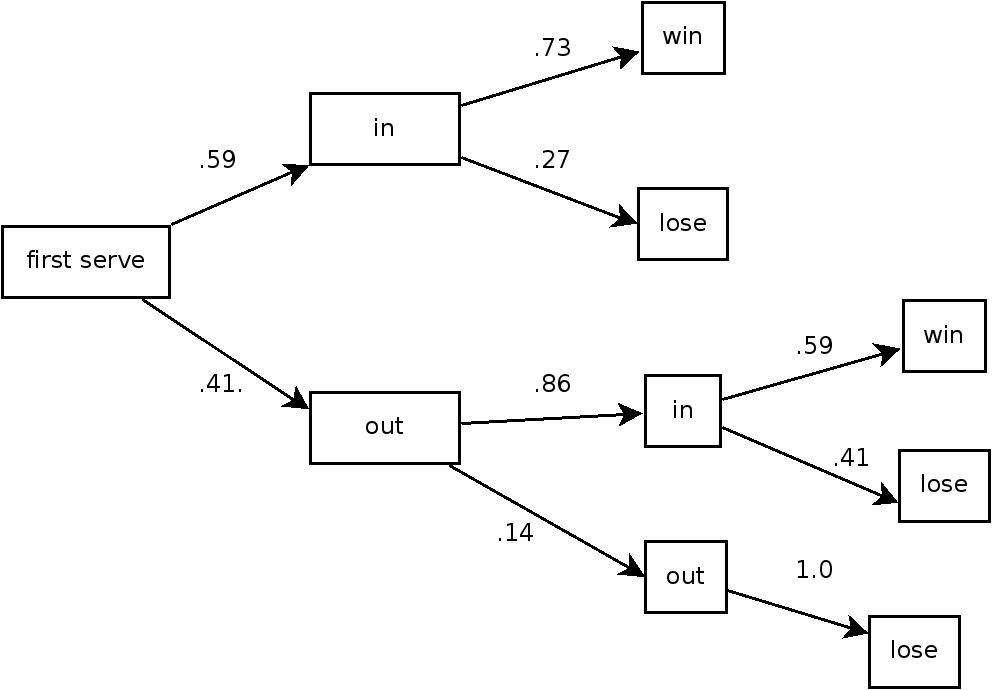
\includegraphics[scale = 0.2]{ex48.jpg}
        \caption{Exercise 48}
      \end{figure}

      The chance of winning by getting the first serve in is:
      \[
        p_{1st} = 0.59 \cdot 0.73 = 0.4307
      \]
      The chance of winning by getting the second serve in is:
      \[
        p_{2nd} = 0.41 \cdot 0.86 \cdot 0.59 = 0.2080
      \]

      Since these two events are disjoint, the probability of the serving player
      winning the point is
      \[
        p_{win} = 0.4307 + 0.2080 \approx \boxed{ 0.6387 }
      \]

    \item[49]
      \begin{figure}[H]
        \centering
        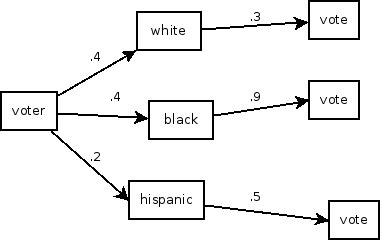
\includegraphics[scale = 0.4]{ex49.jpg}
        \caption{Exercise 49}
      \end{figure}

      \begin{align*}
        p_{white} = 0.4 \cdot 0.3 = 0.12 \\
        p_{black} = 0.4 \cdot 0.9 = 0.36 \\
        p_{hispanic} = 0.2 \cdot 0.5 = 0.1 \\
        \\
        p_{total} = 0.12 + 0.36 + 0.1 = \boxed{ 0.58 } \\
      \end{align*}

    \item[50]
      Given that the server won the point, what was the probability that the first
      serve was in?

      \begin{align*}
        P(\text{in } | \text{ won}) & = \frac{P(\text{in and won})}{P(\text{won})} \\
                    & \approx \frac{0.4307}{0.6387} \\
                    & \approx \boxed{ 0.6743 } \\
      \end{align*}

    \newpage

    \item[51]
      Given that the vote was won, what was the probability that the voter was black?

      \begin{align*}
        P(\text{black } | \text{ won}) & = \frac{P(\text{black and won})}{P(\text{won})} \\
                       & \approx \frac{0.36}{0.58} \\
                       & \approx \boxed{ 0.6207 } \\
      \end{align*}

    \item[54]
      \begin{enumerate}[(a)]
        \item A, B and AB

        \item
          The four combinations you might get are AA, AB, BA, and BB\@. Since there are 
          two ways to get different alleles, this is twice as likely and the probabilities
          are:
          \begin{align*}
            P(A)  & = P(B) = 0.25 \\
            P(AB) & = 0.5 \\
          \end{align*}
      \end{enumerate}

    \item[55]
      \begin{enumerate}[(a)]
        \item B and O

        \item
          The four combinations you might get are BB, BO, OB, and OO\@. There is
          only one way two way to end up with type O and three ways to end up
          with B. The probabilities are
          \begin{align*}
            P(B) & = 0.75 \\
            P(O) & = 0.25 \\
          \end{align*}
      \end{enumerate}

    \item[56]
      \begin{enumerate}[(a)]
        \item 
          With these parents, the possible blood types for the children are: 
          
          A (0.5), AB (0.25), B (0.25)

          The probability of 2 As is 
          \[
            0.5^2 = \boxed{ 0.25 }
          \]

        \item 
          \begin{align*}
            P(same) & = 0.5^2 + 0.25^2 + 0.25^2 \\
                    & = \boxed{ 0.375 }
          \end{align*}
      \end{enumerate}
  \end{description}

  \else
    \vspace{11 cm}
    \begin{quote}
      \begin{em}
        A wrongdoer is often a man who has left something undone, not always one
        who has done something.
      \end{em}
    \end{quote}
    \hspace{1 cm}--Marcus Aurelius
  \fi

\end{document}

